\section{Artificial Intelligence Techniques Applied in This Project}
\label{sec:ai}

This section consolidates the AI methods that underwrite the project---beyond
jurisdiction scoring alone---so that the defence can clearly separate
\emph{domain content} (healthcare regulation) from \emph{technical AI methods}
(representation learning, retrieval, interactive analytics).

\subsection{Role of AI in the Overall System}
\label{sec:ai-role}

Artificial intelligence appears at three layers:
\begin{enumerate}[noitemsep]
  \item \textbf{Object of study:} AI/ML-enabled SaMD and clinical decision support as
        regulated artefacts~\cite{topol2019,rajpurkar2022,esteva2019};
  \item \textbf{Analytical methods:} ordinal multi-theme scoring, composite indices, and
        use-case readiness models (Chapter~\ref{ch:method});
  \item \textbf{Engineering methods:} NLP embeddings, hybrid retrieval, RAG, and
        interactive visualization (Chapter~\ref{ch:rag}).
\end{enumerate}

\subsection{Representation Learning for Regulatory Text}
\label{sec:ai-rep}

Transformer encoders map variable-length text $x$ to dense vectors
$\mathbf{e}=f_\theta(x)\in\mathbb{R}^{d}$~\cite{vaswani2017,devlin2019}. Self-attention
allows the model to relate distant tokens (e.g., ``high-risk'' and ``medical device'')
without handcrafted features. Domain-adapted checkpoints such as SciBERT improve
scientific vocabulary coverage~\cite{beltagy2019}. In this project, embeddings support:
\begin{itemize}[noitemsep]
  \item semantic search over guidance documents;
  \item clustering of similar clauses across jurisdictions;
  \item future supervised theme classification with human-in-the-loop labels.
\end{itemize}

\subsection{Classical and Hybrid Information Retrieval}
\label{sec:ai-ir}

Before neural retrieval, BM25 provides a strong sparse baseline that excels at exact
identifiers. Hybrid fusion combines BM25 with dense cosine similarity
(Section~\ref{sec:rag-rrf}, Equation~\eqref{eq:rag-def}). This design choice is deliberate for
defence: it shows mastery of both classical IR and modern dense retrieval rather than
blind reliance on an API chatbot.

\subsection{Retrieval-Augmented Generation}
\label{sec:ai-rag-brief}

RAG conditions a generator on retrieved evidence~\cite{lewis2020rag}, reducing
hallucination risk for statute-sensitive questions. The project treats RAG as a
\emph{systems} contribution: corpus design, chunk metadata, citation policy, and
dashboard integration matter as much as the choice of LLM backbone.

\subsection{Interactive Analytics as Human--AI Collaboration}
\label{sec:ai-hci}

Dashboards are not ``AI'' in the narrow sense of learned predictors, yet they are
central to responsible AI tooling: they externalize model/score assumptions, support
counterfactual theme weighting, and keep humans in control of high-stakes interpretations.
The React and Streamlit interfaces operationalize HITL principles advocated in clinical
AI ethics literature~\cite{char2018,mittelstadt2019}.

\subsection{Deep Learning Context for Clinical AI Regulation}
\label{sec:ai-clinical-dl}

Understanding why regulators struggle with adaptive systems requires brief technical
literacy in deep learning: residual networks and vision transformers dominate medical
imaging pipelines~\cite{he2016,dosovitskiy2021,litjens2017}; sequence models and
transformers underpin clinical NLP~\cite{vaswani2017,devlin2019}. Continuously learning
models motivate lifecycle tools such as Predetermined Change Control Plans
(PCCP)~\cite{fda2023,babic2019,hwang2019}. The compliance themes in this PFE
(validation, transparency, post-market) are therefore mapped to concrete ML failure
modes: distribution shift, opacity, and post-deployment drift.

\subsection{Evaluation Mindset}
\label{sec:ai-eval}

Where a classifier would report F1, this analytics+RAG system reports retrieval
groundedness, citation accuracy, schema coverage, and rank stability under theme
reweighting. The defence message is: \emph{choose metrics that match the artefact}.
Full supervised NLP metrics remain on the roadmap once a labeled clause corpus exists
(Chapter~\ref{ch:conclusion}).

\begin{figure}[htbp]
\centering
\begin{minipage}[t]{0.48\textwidth}
\centering
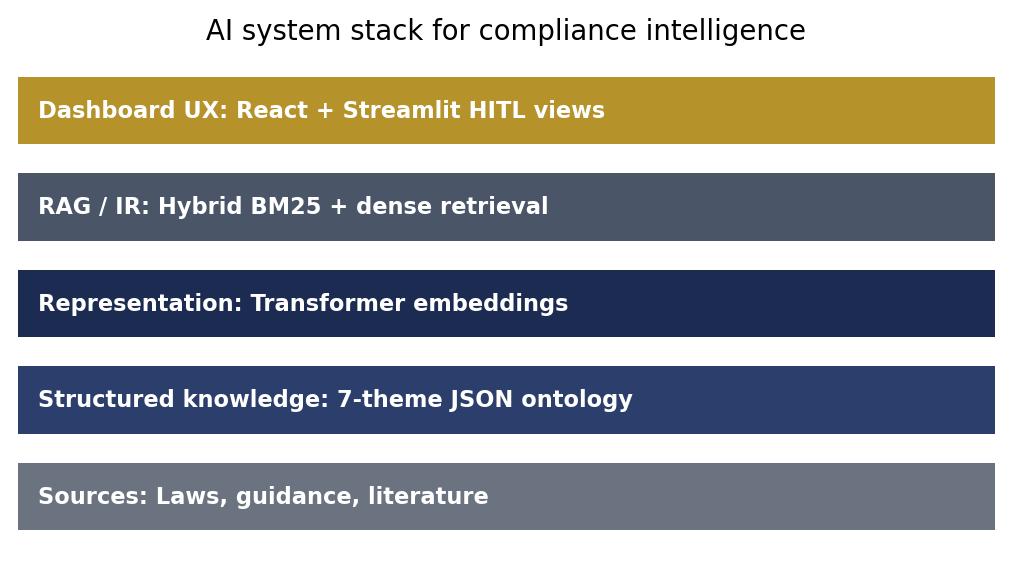
\includegraphics[width=\linewidth]{figures/fig_ai_system_stack.png}
\caption{Layered AI system stack used in this PFE.}
\label{fig:ai-stack}
\end{minipage}\hfill
\begin{minipage}[t]{0.48\textwidth}
\centering
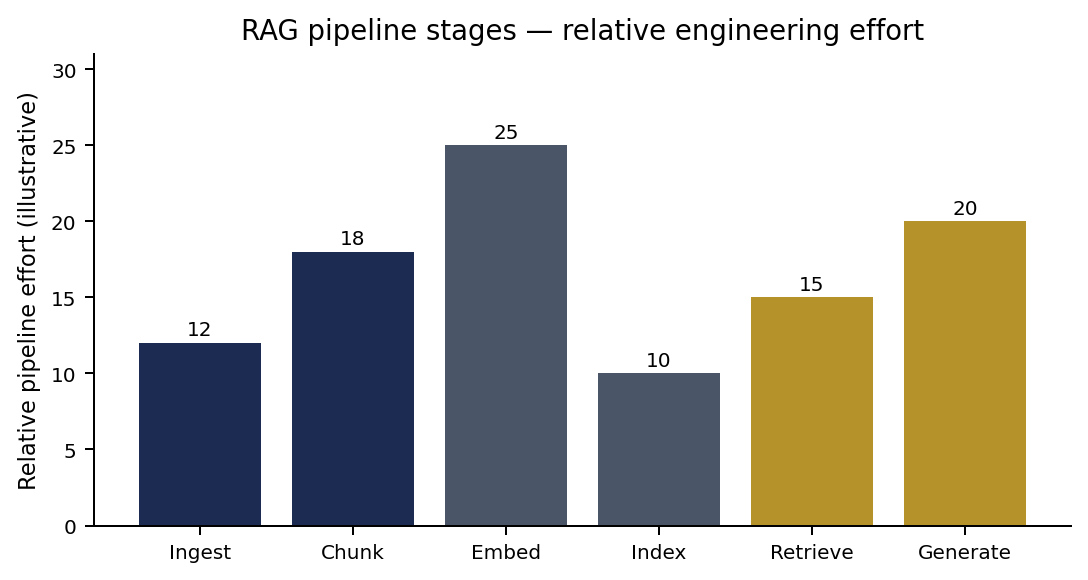
\includegraphics[width=\linewidth]{figures/fig_rag_pipeline_effort.png}
\caption{Illustrative relative engineering effort across RAG stages.}
\label{fig:rag-effort}
\end{minipage}
\end{figure}

